For me it is a ''new'' topic, I know a little bit about it but I dont know as much as I want so a decided to get a deeper knowledge about graphs.

\paragraph{Graph theory}
Is the mathematical theory of the properties and applications of graphs (networks)\\

To understand a little bit more this imagine that you have a set of accesories to wear. Things to put in your head, in ypur body and in your legs. So we need to solve the next question, How many different sets of clothing can I make by choosing an article from each category? Using mathematics we can solve this problem but a graph can help us to solve this visually.

Other common problem is how many friends does the person X have? or how many degrees of separation are there between person X and Y?

\subsection{Types of graphs}

To solve particular problems is necessarilyto know the type of graph that we need to code, and we have different types of graphs each can help us to solve something in particular.

\subsubsection{Undirected graph}
It's the simplest type of graph. An undirected graph is a graph which edges have no orientation. The edge (u, v) is identical to the edge (v, u). Maybe is better if we have a draw:


\begin{figure}[H]
\begin{center}
    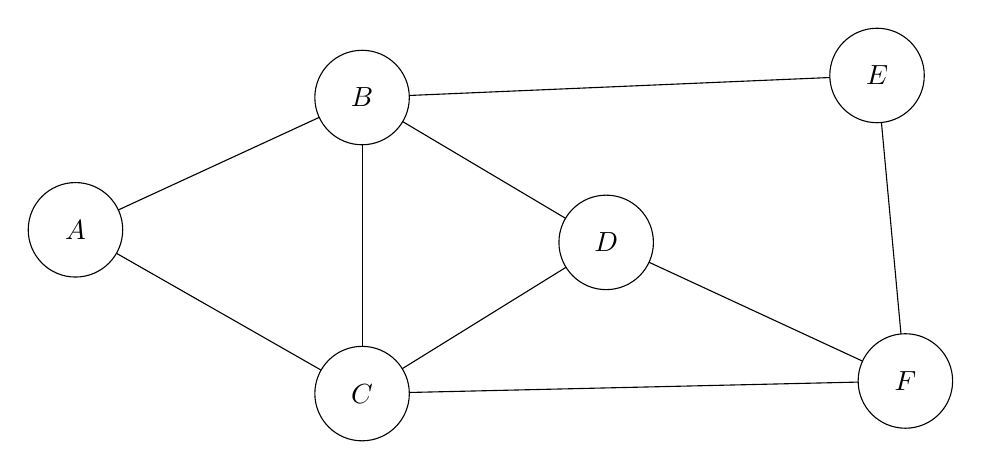
\begin{tikzpicture}[scale=0.2]
    \tikzstyle{every node}+=[inner sep=0pt]
    \draw [black] (8.9,-26.5) circle (3);
    \draw (8.9,-26.5) node {$A$};
    \draw [black] (27.1,-18.1) circle (3);
    \draw (27.1,-18.1) node {$B$};
    \draw [black] (27.1,-36.9) circle (3);
    \draw (27.1,-36.9) node {$C$};
    \draw [black] (42.6,-27.3) circle (3);
    \draw (42.6,-27.3) node {$D$};
    \draw [black] (59.8,-16.7) circle (3);
    \draw (59.8,-16.7) node {$E$};
    \draw [black] (61.6,-36.1) circle (3);
    \draw (61.6,-36.1) node {$F$};
    \draw [black] (11.62,-25.24) -- (24.38,-19.36);
    \draw [black] (11.5,-27.99) -- (24.5,-35.41);
    \draw [black] (29.65,-35.32) -- (40.05,-28.88);
    \draw [black] (29.68,-19.63) -- (40.02,-25.77);
    \draw [black] (27.1,-21.1) -- (27.1,-33.9);
    \draw [black] (30.1,-17.97) -- (56.8,-16.83);
    \draw [black] (45.32,-28.56) -- (58.88,-34.84);
    \draw [black] (60.08,-19.69) -- (61.32,-33.11);
    \draw [black] (30.1,-36.83) -- (58.6,-36.17);
    \end{tikzpicture}
    \caption{Undirected graph diagram}
    \label{fg:undirected-diagram-01}
\end{center}
'\end{figure}

\subsubsection{Directed graph}
A directed graph or digraph is a graph in which edges have orientations. For example, the edge (u, v) is the edge from node u to v.

\begin{figure}[H]
\begin{center}
    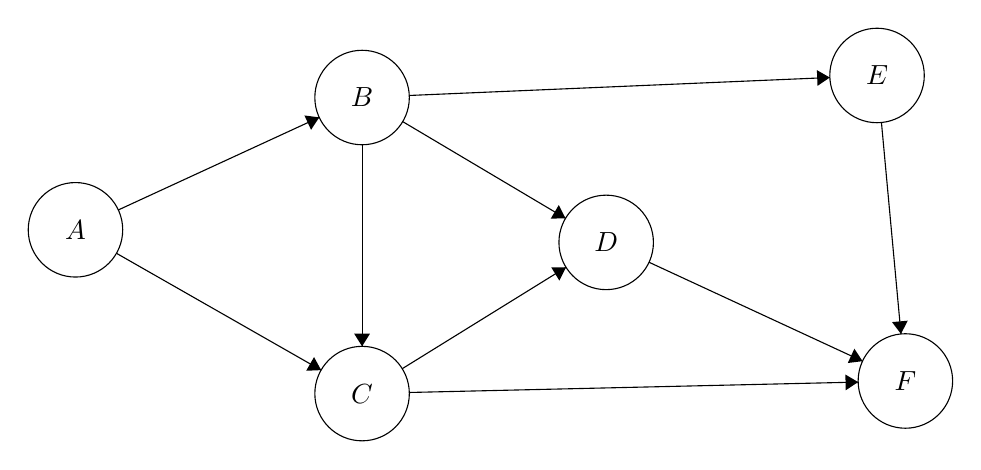
\begin{tikzpicture}[scale=0.2]
    \tikzstyle{every node}+=[inner sep=0pt]
    \draw [black] (8.9,-26.5) circle (3);
    \draw (8.9,-26.5) node {$A$};
    \draw [black] (27.1,-18.1) circle (3);
    \draw (27.1,-18.1) node {$B$};
    \draw [black] (27.1,-36.9) circle (3);
    \draw (27.1,-36.9) node {$C$};
    \draw [black] (42.6,-27.3) circle (3);
    \draw (42.6,-27.3) node {$D$};
    \draw [black] (59.8,-16.7) circle (3);
    \draw (59.8,-16.7) node {$E$};
    \draw [black] (61.6,-36.1) circle (3);
    \draw (61.6,-36.1) node {$F$};
    \draw [black] (11.62,-25.24) -- (24.38,-19.36);
    \fill [black] (24.38,-19.36) -- (23.44,-19.24) -- (23.86,-20.15);
    \draw [black] (11.5,-27.99) -- (24.5,-35.41);
    \fill [black] (24.5,-35.41) -- (24.05,-34.58) -- (23.55,-35.45);
    \draw [black] (29.65,-35.32) -- (40.05,-28.88);
    \fill [black] (40.05,-28.88) -- (39.11,-28.88) -- (39.63,-29.73);
    \draw [black] (29.68,-19.63) -- (40.02,-25.77);
    \fill [black] (40.02,-25.77) -- (39.59,-24.93) -- (39.08,-25.79);
    \draw [black] (27.1,-21.1) -- (27.1,-33.9);
    \fill [black] (27.1,-33.9) -- (27.6,-33.1) -- (26.6,-33.1);
    \draw [black] (30.1,-17.97) -- (56.8,-16.83);
    \fill [black] (56.8,-16.83) -- (55.98,-16.36) -- (56.02,-17.36);
    \draw [black] (45.32,-28.56) -- (58.88,-34.84);
    \fill [black] (58.88,-34.84) -- (58.36,-34.05) -- (57.94,-34.96);
    \draw [black] (60.08,-19.69) -- (61.32,-33.11);
    \fill [black] (61.32,-33.11) -- (61.75,-32.27) -- (60.75,-32.36);
    \draw [black] (30.1,-36.83) -- (58.6,-36.17);
    \fill [black] (58.6,-36.17) -- (57.79,-35.69) -- (57.81,-36.69);
    \end{tikzpicture}
    \caption{Directed graph diagram}
    \label{fg:directed-diagram-01}
\end{center}
\end{figure}

\subsection{Weighted graphs}
Many graphs can have edges that contain a certain weigh to represent an arbitrary value such a cost, distance quantity, etc... 
Something important to know is that an edge will be represented as a triplet (u, v, w) and specify whether the graph is directed or undirected.

\begin{figure}[H]
\begin{center}
    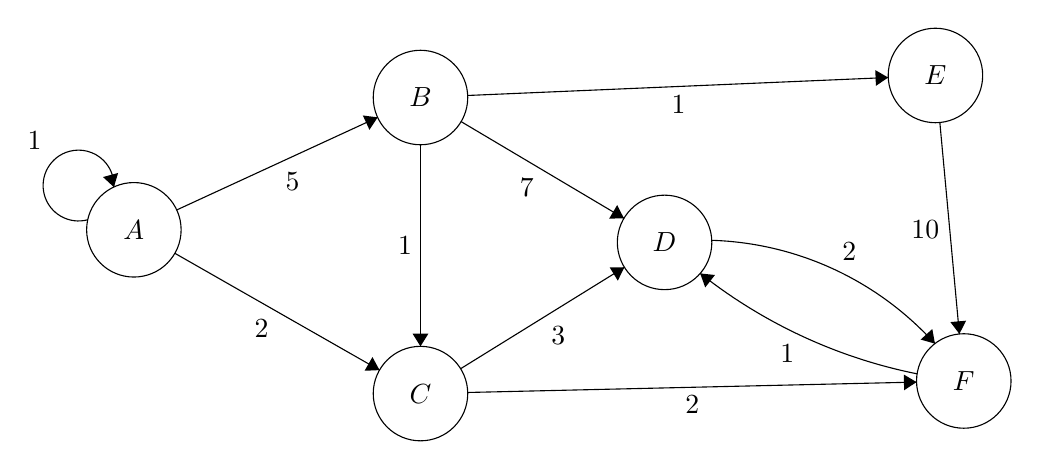
\begin{tikzpicture}[scale=0.2]
    \tikzstyle{every node}+=[inner sep=0pt]
    \draw [black] (8.9,-26.5) circle (3);
    \draw (8.9,-26.5) node {$A$};
    \draw [black] (27.1,-18.1) circle (3);
    \draw (27.1,-18.1) node {$B$};
    \draw [black] (27.1,-36.9) circle (3);
    \draw (27.1,-36.9) node {$C$};
    \draw [black] (42.6,-27.3) circle (3);
    \draw (42.6,-27.3) node {$D$};
    \draw [black] (59.8,-16.7) circle (3);
    \draw (59.8,-16.7) node {$E$};
    \draw [black] (61.6,-36.1) circle (3);
    \draw (61.6,-36.1) node {$F$};
    \draw [black] (11.62,-25.24) -- (24.38,-19.36);
    \fill [black] (24.38,-19.36) -- (23.44,-19.24) -- (23.86,-20.15);
    \draw (18.98,-22.81) node [below] {$5$};
    \draw [black] (11.5,-27.99) -- (24.5,-35.41);
    \fill [black] (24.5,-35.41) -- (24.05,-34.58) -- (23.55,-35.45);
    \draw (17,-32.2) node [below] {$2$};
    \draw [black] (29.65,-35.32) -- (40.05,-28.88);
    \fill [black] (40.05,-28.88) -- (39.11,-28.88) -- (39.63,-29.73);
    \draw (35.85,-32.6) node [below] {$3$};
    \draw [black] (29.68,-19.63) -- (40.02,-25.77);
    \fill [black] (40.02,-25.77) -- (39.59,-24.93) -- (39.08,-25.79);
    \draw (33.85,-23.2) node [below] {$7$};
    \draw [black] (27.1,-21.1) -- (27.1,-33.9);
    \fill [black] (27.1,-33.9) -- (27.6,-33.1) -- (26.6,-33.1);
    \draw (26.6,-27.5) node [left] {$1$};
    \draw [black] (30.1,-17.97) -- (56.8,-16.83);
    \fill [black] (56.8,-16.83) -- (55.98,-16.36) -- (56.02,-17.36);
    \draw (43.49,-17.94) node [below] {$1$};
    \draw [black] (45.594,-27.167) arc (88.2315:42.06533:19.916);
    \fill [black] (59.77,-33.73) -- (59.6,-32.8) -- (58.86,-33.47);
    \draw (54.33,-28.49) node [above] {$2$};
    \draw [black] (60.08,-19.69) -- (61.32,-33.11);
    \fill [black] (61.32,-33.11) -- (61.75,-32.27) -- (60.75,-32.36);
    \draw (60.07,-26.48) node [left] {$10$};
    \draw [black] (30.1,-36.83) -- (58.6,-36.17);
    \fill [black] (58.6,-36.17) -- (57.79,-35.69) -- (57.81,-36.69);
    \draw (44.36,-37.02) node [below] {$2$};
    \draw [black] (5.981,-25.859) arc (285.34019:-2.65981:2.25);
    \draw (3.07,-20.86) node [left] {$1$};
    \fill [black] (7.63,-23.79) -- (7.9,-22.89) -- (6.94,-23.15);
    \draw [black] (58.636,-35.646) arc (-101.35141:-128.35177:32.507);
    \fill [black] (44.86,-29.27) -- (45.18,-30.16) -- (45.8,-29.37);
    \draw (50.39,-33.78) node [below] {$1$};
    \end{tikzpicture}
    \caption{Weighted graph diagram}
    \label{fg:weighted-diagram-01}
\end{center}
\end{figure}

\subsection{Directed acyclic graphs (DAGs)}
DAGs are directed graphs with no cycles. These graphs play an important role in representing structures with dependencies. Several efficient algorithms exits to operates on DAGs.
\textbf{IMPORTANT:} All out-trees are DAGs but not all DAGs are out-trees.

\begin{figure}[H]
\begin{center}
    \begin{tikzpicture}[scale=0.2]
    \tikzstyle{every node}+=[inner sep=0pt]
    \draw [black] (4.6,-25.8) circle (3);
    \draw [black] (20.1,-12) circle (3);
    \draw [black] (20.1,-39.8) circle (3);
    \draw [black] (35.2,-25.8) circle (3);
    \draw [black] (54.1,-12) circle (3);
    \draw [black] (54.1,-25.8) circle (3);
    \draw [black] (54.1,-39.8) circle (3);
    \draw [black] (73,-25.8) circle (3);
    \draw [black] (6.84,-23.81) -- (17.86,-13.99);
    \fill [black] (17.86,-13.99) -- (16.93,-14.15) -- (17.59,-14.9);
    \draw [black] (6.83,-27.81) -- (17.87,-37.79);
    \fill [black] (17.87,-37.79) -- (17.62,-36.88) -- (16.94,-37.62);
    \draw [black] (20.1,-15) -- (20.1,-36.8);
    \fill [black] (20.1,-36.8) -- (20.6,-36) -- (19.6,-36);
    \draw [black] (22.31,-14.02) -- (32.99,-23.78);
    \fill [black] (32.99,-23.78) -- (32.73,-22.87) -- (32.06,-23.61);
    \draw [black] (22.3,-37.76) -- (33,-27.84);
    \fill [black] (33,-27.84) -- (32.07,-28.02) -- (32.75,-28.75);
    \draw [black] (37.62,-24.03) -- (51.68,-13.77);
    \fill [black] (51.68,-13.77) -- (50.74,-13.84) -- (51.33,-14.64);
    \draw [black] (37.61,-27.59) -- (51.69,-38.01);
    \fill [black] (51.69,-38.01) -- (51.34,-37.14) -- (50.75,-37.94);
    \draw [black] (38.2,-25.8) -- (51.1,-25.8);
    \fill [black] (51.1,-25.8) -- (50.3,-25.3) -- (50.3,-26.3);
    \draw [black] (56.52,-13.77) -- (70.58,-24.03);
    \fill [black] (70.58,-24.03) -- (70.23,-23.16) -- (69.64,-23.96);
    \draw [black] (57.1,-25.8) -- (70,-25.8);
    \fill [black] (70,-25.8) -- (69.2,-25.3) -- (69.2,-26.3);
    \draw [black] (56.51,-38.01) -- (70.59,-27.59);
    \fill [black] (70.59,-27.59) -- (69.65,-27.66) -- (70.24,-28.46);
    \draw [black] (23.1,-12) -- (51.1,-12);
    \fill [black] (51.1,-12) -- (50.3,-11.5) -- (50.3,-12.5);
    \draw [black] (23.1,-39.8) -- (51.1,-39.8);
    \fill [black] (51.1,-39.8) -- (50.3,-39.3) -- (50.3,-40.3);
    \end{tikzpicture}
    \caption{Directed Acyclic graph diagram}
    \label{fg:DAGs-diagram-01}
\end{center}
\end{figure}    

\subsection{Bipartite graph}
A bipartite graph is one whose vertices can be split into two independent groups U, V such that every edge connects betweens U and V.

Other definitions exist such as: the graph is two colourable or there is no odd lenght cycle.
\begin{figure}[H]
\begin{center}
    \begin{tikzpicture}[scale=0.2]
    \tikzstyle{every node}+=[inner sep=0pt]
    \draw [black] (4.5,-4.5) circle (3);
    \draw [black] (4.5,-4.5) circle (2.4);
    \draw [black] (74.6,-4.5) circle (3);
    \draw [black] (32.4,-22.2) circle (3);
    \draw [black] (48.5,-22.2) circle (3);
    \draw [black] (48.5,-22.2) circle (2.4);
    \draw [black] (32.4,-37.6) circle (3);
    \draw [black] (32.4,-37.6) circle (2.4);
    \draw [black] (48.5,-37.6) circle (3);
    \draw [black] (4.5,-55.3) circle (3);
    \draw [black] (74.6,-55.3) circle (3);
    \draw [black] (74.6,-55.3) circle (2.4);
    \draw [black] (35.4,-22.2) -- (45.5,-22.2);
    \draw [black] (48.5,-25.2) -- (48.5,-34.6);
    \draw [black] (45.5,-37.6) -- (35.4,-37.6);
    \draw [black] (32.4,-34.6) -- (32.4,-25.2);
    \draw [black] (72.12,-6.18) -- (50.98,-20.52);
    \draw [black] (7.03,-6.11) -- (29.87,-20.59);
    \draw [black] (7.03,-53.69) -- (29.87,-39.21);
    \draw [black] (72.12,-53.62) -- (50.98,-39.28);
    \draw [black] (7.5,-4.5) -- (71.6,-4.5);
    \draw [black] (74.6,-7.5) -- (74.6,-52.3);
    \draw [black] (71.6,-55.3) -- (7.5,-55.3);
    \draw [black] (4.5,-52.3) -- (4.5,-7.5);
    \end{tikzpicture}
    \caption{Bipartite graph diagram 01}
    \label{fg:bipartite-graph-01}
\end{center}
\end{figure}

\begin{figure}[H]
\begin{center}
    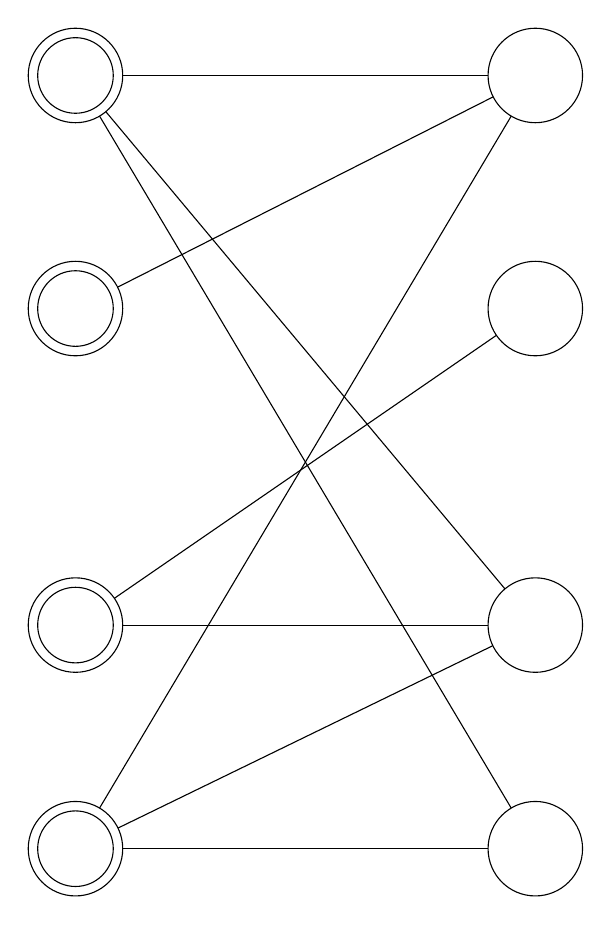
\begin{tikzpicture}[scale=0.2]
    \tikzstyle{every node}+=[inner sep=0pt]
    \draw [black] (23.4,-5.9) circle (3);
    \draw [black] (23.4,-5.9) circle (2.4);
    \draw [black] (23.4,-20.7) circle (3);
    \draw [black] (23.4,-20.7) circle (2.4);
    \draw [black] (23.4,-40.8) circle (3);
    \draw [black] (23.4,-40.8) circle (2.4);
    \draw [black] (23.4,-55) circle (3);
    \draw [black] (23.4,-55) circle (2.4);
    \draw [black] (52.6,-5.9) circle (3);
    \draw [black] (52.6,-20.7) circle (3);
    \draw [black] (52.6,-40.8) circle (3);
    \draw [black] (52.6,-55) circle (3);
    \draw [black] (26.4,-5.9) -- (49.6,-5.9);
    \draw [black] (26.4,-55) -- (49.6,-55);
    \draw [black] (25.33,-8.2) -- (50.67,-38.5);
    \draw [black] (24.93,-8.48) -- (51.07,-52.42);
    \draw [black] (49.92,-7.26) -- (26.08,-19.34);
    \draw [black] (51.07,-8.48) -- (24.93,-52.42);
    \draw [black] (50.13,-22.4) -- (25.87,-39.1);
    \draw [black] (49.6,-40.8) -- (26.4,-40.8);
    \draw [black] (49.9,-42.11) -- (26.1,-53.69);
    \end{tikzpicture}
    \caption{Bipartite graph diagram 02}
    \label{fg:bipartite-graph-02}
\end{center}
\end{figure}

\subsection{Complete graphs}
A complete graph is one where there is a unique edge between every pair of nodes. A complete graph with n vertices is denoted as the graph $K_{n}$
\begin{figure}[H]
\begin{center}
    \begin{tikzpicture}[scale=0.2]
    \tikzstyle{every node}+=[inner sep=0pt]
    \draw [black] (5.8,-25) circle (3);
    \draw [black] (19.6,-20.2) circle (3);
    \draw [black] (19.6,-32.6) circle (3);
    \draw [black] (32.3,-20.2) circle (3);
    \draw [black] (44.1,-26.8) circle (3);
    \draw [black] (32.3,-32.6) circle (3);
    \draw [black] (54.9,-18.9) circle (3);
    \draw [black] (72.4,-18.9) circle (3);
    \draw [black] (54.9,-34.4) circle (3);
    \draw [black] (72.4,-34.4) circle (3);
    \draw [white] (5.8,-44.7) circle (3);
    \draw (5.8,-44.7) node {$K_1$};
    \draw [white] (19.6,-44.7) circle (3);
    \draw (19.6,-44.7) node {$K_2$};
    \draw [white] (36.6,-44.7) circle (3);
    \draw (36.6,-44.7) node {$K_3$};
    \draw [white] (63.2,-44.7) circle (3);
    \draw (63.2,-44.7) node {$K_4$};
    \draw [black] (19.6,-23.2) -- (19.6,-29.6);
    \draw [black] (32.3,-29.6) -- (32.3,-23.2);
    \draw [black] (34.92,-21.66) -- (41.48,-25.34);
    \draw [black] (34.99,-31.28) -- (41.41,-28.12);
    \draw [black] (57.9,-18.9) -- (69.4,-18.9);
    \draw [black] (57.9,-34.4) -- (69.4,-34.4);
    \draw [black] (54.9,-21.9) -- (54.9,-31.4);
    \draw [black] (72.4,-21.9) -- (72.4,-31.4);
    \draw [black] (57.15,-20.89) -- (70.15,-32.41);
    \draw [black] (57.15,-32.41) -- (70.15,-20.89);
    \end{tikzpicture}
    \caption{Complete graph diagram}
    \label{fg:complete-graph-diagram-01}
\end{center}        
\end{figure}

\subsection{¿How can we represent a graph?}
\subsubsection{Adjacency Matrix}
An adjacency matrix m is a very simple way to represent a graph. The idea is that the cell $m[i][j]$ represents the edge weigh of going from node i to node j.
Let's suppose that we have the next graph:

\begin{figure}[H]
\begin{center}
    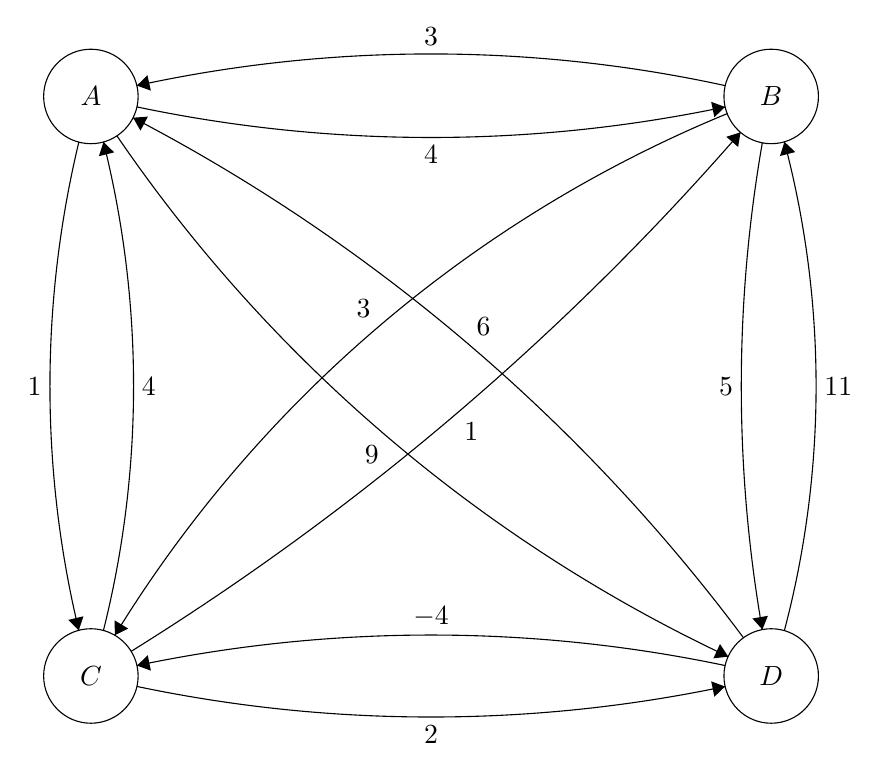
\begin{tikzpicture}[scale=0.2]
    \tikzstyle{every node}+=[inner sep=0pt]
    \draw [black] (15.4,-12.1) circle (3);
    \draw (15.4,-12.1) node {$A$};
    \draw [black] (58.6,-12.1) circle (3);
    \draw (58.6,-12.1) node {$B$};
    \draw [black] (15.4,-48.9) circle (3);
    \draw (15.4,-48.9) node {$C$};
    \draw [black] (58.6,-48.9) circle (3);
    \draw (58.6,-48.9) node {$D$};
    \draw [black] (14.634,-46) arc (-166.49637:-193.50363:66.378);
    \fill [black] (14.63,-46) -- (14.93,-45.11) -- (13.96,-45.34);
    \draw (12.3,-30.5) node [left] {$1$};
    \draw [black] (55.675,-12.765) arc (-78.13087:-101.86913:90.797);
    \fill [black] (55.67,-12.77) -- (54.79,-12.44) -- (54.99,-13.42);
    \draw (37,-15.21) node [below] {$4$};
    \draw [black] (58.036,-45.954) arc (-170.11327:-189.88673:90.004);
    \fill [black] (58.04,-45.95) -- (58.39,-45.08) -- (57.41,-45.25);
    \draw (56.2,-30.5) node [left] {$5$};
    \draw [black] (55.675,-49.565) arc (-78.13087:-101.86913:90.797);
    \fill [black] (55.67,-49.57) -- (54.79,-49.24) -- (54.99,-50.22);
    \draw (37,-52.01) node [below] {$2$};
    \draw [black] (18.32,-11.411) arc (102.29223:77.70777:87.743);
    \fill [black] (18.32,-11.41) -- (19.21,-11.73) -- (18.99,-10.75);
    \draw (37,-8.9) node [above] {$3$};
    \draw [black] (18.325,-48.236) arc (101.84794:78.15206:90.956);
    \fill [black] (18.33,-48.24) -- (19.21,-48.56) -- (19.01,-47.58);
    \draw (37,-45.8) node [above] {$-4$};
    \draw [black] (16.197,-14.992) arc (14.07018:-14.07018:63.791);
    \fill [black] (16.2,-14.99) -- (15.91,-15.89) -- (16.88,-15.65);
    \draw (18.61,-30.5) node [right] {$4$};
    \draw [black] (55.866,-47.666) arc (-115.16899:-145.68317:96.876);
    \fill [black] (55.87,-47.67) -- (55.35,-46.87) -- (54.93,-47.78);
    \draw (33.24,-34.23) node [below] {$9$};
    \draw [black] (18.077,-13.453) arc (62.43021:36.71764:114.419);
    \fill [black] (18.08,-13.45) -- (18.55,-14.27) -- (19.02,-13.38);
    \draw (40.33,-27.29) node [above] {$6$};
    \draw [black] (16.921,-46.314) arc (148.48548:112.36668:82.386);
    \fill [black] (16.92,-46.31) -- (17.77,-45.89) -- (16.91,-45.37);
    \draw (32.72,-26.17) node [above] {$3$};
    \draw [black] (56.651,-14.381) arc (-41.01318:-58.13466:170.714);
    \fill [black] (56.65,-14.38) -- (55.75,-14.66) -- (56.5,-15.31);
    \draw (39.55,-32.8) node [below] {$1$};
    \draw [black] (59.437,-14.98) arc (14.79508:-14.79508:60.775);
    \fill [black] (59.44,-14.98) -- (59.16,-15.88) -- (60.13,-15.63);
    \draw (61.95,-30.5) node [right] {$11$};
    \end{tikzpicture}
\end{center}        
\end{figure}

If we build an adjacency matrix using the graph above, we have the next as a result
$
    \begin{bheadmatrix}[A & B &C &D][*{4}{r}]
        0 & 4 & 1 & 9 \\
        3 & 0 & 6 & 11 \\
        4 & 1 & 0 & 2\\
        6 & 5 & -4 & 0
    \end{bheadmatrix}%    
$

\textbf{NOTE:} It is often assumed that the edge of going from a node to itself has a cost of zero.\\

Now we need to know why is better or not to use an adjacency matrix

\begin{table}[H]
    \centering
    \resizebox{\textwidth}{!}{%
    \begin{tabular}{ll}
    \hline
    \rowcolor[HTML]{00009B} 
    {\color[HTML]{FFFFFF} Pros}                                                                & {\color[HTML]{FFFFFF} Cons}                                                              \\ \hline
    \begin{tabular}[c]{@{}l@{}}Space eifficient for representating dense\\ graphs\end{tabular} & Requires $O(V^{2})$ space                                                                \\ \hline
    Edge weight lookup is $O(1)$                                                               & \begin{tabular}[c]{@{}l@{}}Iterating over all edges takes\\ $O(V^{2})$ time\end{tabular} \\ \hline
    Simplest graph representation                                                              &                                                                                          \\ \hline
    \end{tabular}%
    }
\end{table}

\subsubsection{Adjacency list}
An adjacency list is a way to represent a graph as a map from nodes to lists of edges

\begin{figure}[H]
\begin{center}
    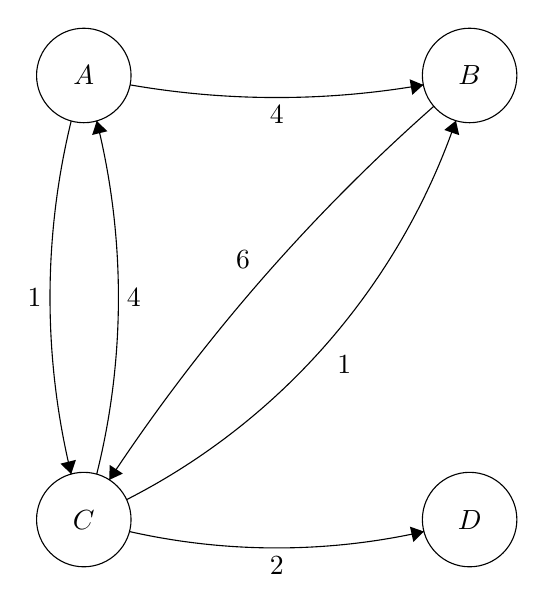
\begin{tikzpicture}[scale=0.2]
    \tikzstyle{every node}+=[inner sep=0pt]
    \draw [black] (29.4,-14.8) circle (3);
    \draw (29.4,-14.8) node {$A$};
    \draw [black] (53.9,-14.8) circle (3);
    \draw (53.9,-14.8) node {$B$};
    \draw [black] (29.4,-43) circle (3);
    \draw (29.4,-43) node {$C$};
    \draw [black] (53.9,-43) circle (3);
    \draw (53.9,-43) node {$D$};
    \draw [black] (28.598,-40.11) arc (-166.31538:-193.68462:47.382);
    \fill [black] (28.6,-40.11) -- (28.9,-39.21) -- (27.92,-39.45);
    \draw (26.75,-28.9) node [left] {$1$};
    \draw [black] (50.96,-15.397) arc (-80.11315:-99.88685:54.223);
    \fill [black] (50.96,-15.4) -- (50.09,-15.04) -- (50.26,-16.03);
    \draw (41.65,-16.7) node [below] {$4$};
    \draw [black] (50.999,-43.762) arc (-77.30143:-102.69857:42.53);
    \fill [black] (51,-43.76) -- (50.11,-43.45) -- (50.33,-44.43);
    \draw (41.65,-45.3) node [below] {$2$};
    \draw [black] (30.221,-17.685) arc (14.02278:-14.02278:46.284);
    \fill [black] (30.22,-17.69) -- (29.93,-18.58) -- (30.9,-18.34);
    \draw (32.1,-28.9) node [right] {$4$};
    \draw [black] (53.027,-17.669) arc (-18.94912:-63.01873:42.486);
    \fill [black] (53.03,-17.67) -- (52.29,-18.26) -- (53.24,-18.59);
    \draw (45.46,-33.19) node [right] {$1$};
    \draw [black] (31.02,-40.475) arc (146.59593:131.43622:119.096);
    \fill [black] (31.02,-40.48) -- (31.88,-40.08) -- (31.04,-39.53);
    \draw (39.99,-26.48) node [left] {$6$};
    \end{tikzpicture}
\end{center}        
\end{figure}

If we made a list we have the next as a result: 

A -> [(B, 4), (C,1)]\par
B -> [(C,6)]\par
C -> [(A,4),(B,1),(D,2)]\par
D -> []\par

Let's take the node C as an example. As we can see the node C can reach with nodes:
\begin{itemize}
    \item {Node A with cost 4}
    \item {Node B with cost 1}
    \item {Node D with cost 2}
\end{itemize}

As we made with the adjacency matrix we have some cons and pros for this representation:

\begin{table}[H]
    \centering
    \resizebox{\textwidth}{!}{%
    \begin{tabular}{ll}
    \hline
    \rowcolor[HTML]{00009B} 
    {\color[HTML]{FFFFFF} Pros}                                                                & {\color[HTML]{FFFFFF} Cons}                                                          \\ \hline
    \begin{tabular}[c]{@{}l@{}}Space efficient for representating\\ sparse graphs\end{tabular} & \begin{tabular}[c]{@{}l@{}}Less space efficient for denser\\ graphs\end{tabular}     \\ \hline
    Iterating over all edges is efficient                                                      & Edge weight lookup is $O(E)$                                                         \\ \hline
                                                                                               & \begin{tabular}[c]{@{}l@{}}Slightly more complex graph\\ representation\end{tabular} \\ \hline
    \end{tabular}%
    }
\end{table}

\subsubsection{Edge list}
An edge list is a way to represent a graph simply as an unordered list of edges. Assume the notation for any triplet (u, v, w) means:
''the cost from node u to node v is w''

If we take the same graph as the adjacent list and make a transformation of this graph to an edge list we get the next:

\[
    [(C,A,4), (A,C,1), (B,C,6), (A,B,4), (C,B,1), (C,D,2)]
\]

This representation is seldomly used because of its lack of structure. However, it is conceptually simple and practical in a handful algorithms.

As the last representations we have some cons and pros for the edge list:

\begin{table}[]
    \centering
    \resizebox{\textwidth}{!}{%
    \begin{tabular}{ll}
    \hline
    \rowcolor[HTML]{00009B} 
    {\color[HTML]{FFFFFF} Pros}                                                              & {\color[HTML]{FFFFFF} Cons}                                                      \\ \hline
    \begin{tabular}[c]{@{}l@{}}Space efficient for representing\\ sparse graphs\end{tabular} & \begin{tabular}[c]{@{}l@{}}Less space efficient for denser\\ graphs\end{tabular} \\ \hline
    Iterating over all edges is efficient                                                    & Edge weight lookup is $O(E)$                                                     \\ \hline
    Very simple structure                                                                    &                                                                                  \\ \hline
    \end{tabular}%
    }
\end{table}

\subsection{Common graph theory problems}

\subsubsection{How can we solve graph theory problems?}
Is necessarily ask yourself:
\begin{enumerate}
    \item {Is the graph directed or undirected?}
    \item {Are the edges of the graph weighted?}
    \item {Is the graph I will encounter likely to be sparse or dense with edges?}
    \item {Should I use an adjacency matrix, adjacency list, an edge list or other structure to represent the graph efficiently?}
\end{enumerate}

\subsubsection{Shortest path problem}
Given a weighted graph, find the shortest path of edges from node A to node B.

\begin{figure}[H]
\begin{center}
    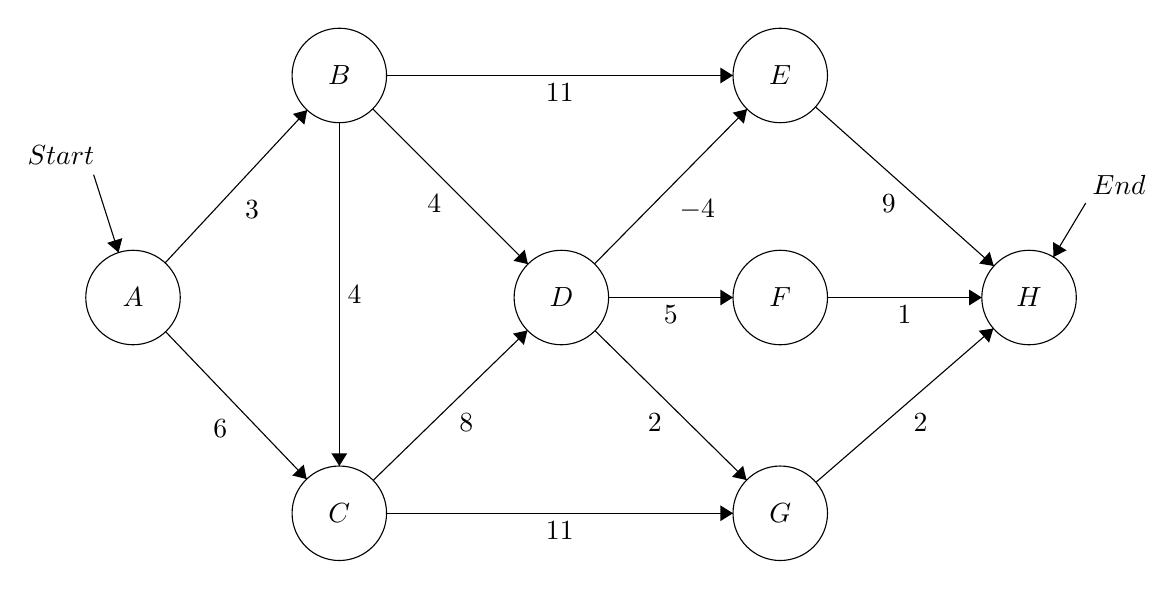
\begin{tikzpicture}[scale=0.2]
    \tikzstyle{every node}+=[inner sep=0pt]
    \draw [black] (9,-26.9) circle (3);
    \draw (9,-26.9) node {$A$};
    \draw [black] (22.1,-12.8) circle (3);
    \draw (22.1,-12.8) node {$B$};
    \draw [black] (22.1,-40.6) circle (3);
    \draw (22.1,-40.6) node {$C$};
    \draw [black] (36.2,-26.9) circle (3);
    \draw (36.2,-26.9) node {$D$};
    \draw [black] (50.1,-12.8) circle (3);
    \draw (50.1,-12.8) node {$E$};
    \draw [black] (50.1,-26.9) circle (3);
    \draw (50.1,-26.9) node {$F$};
    \draw [black] (50.1,-40.6) circle (3);
    \draw (50.1,-40.6) node {$G$};
    \draw [black] (65.9,-26.9) circle (3);
    \draw (65.9,-26.9) node {$H$};
    \draw [black] (11.04,-24.7) -- (20.06,-15);
    \fill [black] (20.06,-15) -- (19.15,-15.24) -- (19.88,-15.92);
    \draw (16.08,-21.31) node [right] {$3$};
    \draw [black] (11.07,-29.07) -- (20.03,-38.43);
    \fill [black] (20.03,-38.43) -- (19.84,-37.51) -- (19.11,-38.2);
    \draw (15.02,-35.22) node [left] {$6$};
    \draw [black] (22.1,-15.8) -- (22.1,-37.6);
    \fill [black] (22.1,-37.6) -- (22.6,-36.8) -- (21.6,-36.8);
    \draw (22.6,-26.7) node [right] {$4$};
    \draw [black] (24.22,-14.92) -- (34.08,-24.78);
    \fill [black] (34.08,-24.78) -- (33.87,-23.86) -- (33.16,-24.57);
    \draw (28.13,-20.33) node [below] {$4$};
    \draw [black] (24.25,-38.51) -- (34.05,-28.99);
    \fill [black] (34.05,-28.99) -- (33.13,-29.19) -- (33.82,-29.91);
    \draw (30.17,-34.23) node [below] {$8$};
    \draw [black] (25.1,-12.8) -- (47.1,-12.8);
    \fill [black] (47.1,-12.8) -- (46.3,-12.3) -- (46.3,-13.3);
    \draw (36.1,-13.3) node [below] {$11$};
    \draw [black] (25.1,-40.6) -- (47.1,-40.6);
    \fill [black] (47.1,-40.6) -- (46.3,-40.1) -- (46.3,-41.1);
    \draw (36.1,-41.1) node [below] {$11$};
    \draw [black] (38.31,-24.76) -- (47.99,-14.94);
    \fill [black] (47.99,-14.94) -- (47.08,-15.16) -- (47.79,-15.86);
    \draw (43.68,-21.32) node [right] {$-4$};
    \draw [black] (38.34,-29.01) -- (47.96,-38.49);
    \fill [black] (47.96,-38.49) -- (47.74,-37.58) -- (47.04,-38.29);
    \draw (42.13,-34.23) node [below] {$2$};
    \draw [black] (39.2,-26.9) -- (47.1,-26.9);
    \fill [black] (47.1,-26.9) -- (46.3,-26.4) -- (46.3,-27.4);
    \draw (43.15,-27.4) node [below] {$5$};
    \draw [black] (53.1,-26.9) -- (62.9,-26.9);
    \fill [black] (62.9,-26.9) -- (62.1,-26.4) -- (62.1,-27.4);
    \draw (58,-27.4) node [below] {$1$};
    \draw [black] (52.34,-14.8) -- (63.66,-24.9);
    \fill [black] (63.66,-24.9) -- (63.4,-24) -- (62.73,-24.74);
    \draw (56.99,-20.34) node [below] {$9$};
    \draw [black] (52.37,-38.63) -- (63.63,-28.87);
    \fill [black] (63.63,-28.87) -- (62.7,-29.01) -- (63.36,-29.77);
    \draw (59.01,-34.24) node [below] {$2$};
    \draw [black] (6.5,-19.1) -- (8.08,-24.04);
    \draw (4.42,-18.5) node [above] {$Start$};
    \fill [black] (8.08,-24.04) -- (8.32,-23.13) -- (7.36,-23.43);
    \draw [black] (69.5,-20.9) -- (67.44,-24.33);
    \draw (71.61,-20.4) node [above] {$End$};
    \fill [black] (67.44,-24.33) -- (68.28,-23.9) -- (67.43,-23.38);
    \end{tikzpicture}
\end{center}        
\end{figure}

Using the example above we can see that the sortest path with the minimum cost is $A \rightarrow B \rightarrow D \rightarrow G \rightarrow H$\\

\textbf{Algorithms:} BFS (unweighted graph), Dijkstra's, Bellman-Ford, Floyd-Warshall, A*, and many more...

\subsubsection{Connectivity}

Does there exist a path between node A and node B?

\begin{figure}[H]
\begin{center}
    \begin{tikzpicture}[scale=0.2]
    \tikzstyle{every node}+=[inner sep=0pt]
    \draw [black] (10.7,-5.8) circle (3);
    \draw [black] (6.1,-15.4) circle (3);
    \draw [black] (19,-14.2) circle (3);
    \draw [black] (25.3,-24.2) circle (3);
    \draw [black] (37.7,-27.8) circle (3);
    \draw [black] (47.2,-22.6) circle (3);
    \draw [black] (38.7,-17.3) circle (3);
    \draw [black] (45.6,-7.3) circle (3);
    \draw [black] (70.9,-14.5) circle (3);
    \draw [black] (68.2,-25.8) circle (3);
    \draw [black] (77.9,-22.6) circle (3);
    \draw [black] (60.1,-32.2) circle (3);
    \draw [black] (24.5,-38.4) circle (3);
    \draw [black] (22.2,-51.8) circle (3);
    \draw [black] (36.7,-44.4) circle (3);
    \draw [black] (45.8,-52.7) circle (3);
    \draw [black] (54.5,-42.2) circle (3);
    \draw [black] (7.3,-40) circle (3);
    \draw [black] (9.4,-8.51) -- (7.4,-12.69);
    \draw [black] (9.09,-15.12) -- (16.01,-14.48);
    \draw [black] (12.81,-7.93) -- (16.89,-12.07);
    \draw [black] (40.4,-14.83) -- (43.9,-9.77);
    \draw [black] (44.65,-21.01) -- (41.25,-18.89);
    \draw [black] (40.33,-26.36) -- (44.57,-24.04);
    \draw [black] (38.42,-20.29) -- (37.98,-24.81);
    \draw [black] (28.18,-25.04) -- (34.82,-26.96);
    \draw [black] (70.2,-17.42) -- (68.9,-22.88);
    \draw [black] (75.05,-23.54) -- (71.05,-24.86);
    \draw [black] (65.85,-27.66) -- (62.45,-30.34);
    \draw [black] (34.01,-43.08) -- (27.19,-39.72);
    \draw [black] (34.03,-45.76) -- (24.87,-50.44);
    \draw [black] (23.99,-41.36) -- (22.71,-48.84);
    \draw [black] (25.2,-51.91) -- (42.8,-52.59);
    \draw [black] (38.92,-46.42) -- (43.58,-50.68);
    \draw [black] (51.52,-42.57) -- (39.68,-44.03);
    \draw [black] (52.59,-44.51) -- (47.71,-50.39);
    \end{tikzpicture}
\end{center}        
\end{figure}

\textbf{Tipical solution:} Use union find data structure or any search algorithm (e.g. DFS)

\subsubsection{Negative cycles}
Does my weighted digraph (directed graph) have any negative cycles? if so, where?

\begin{figure}[H]
\begin{center}
    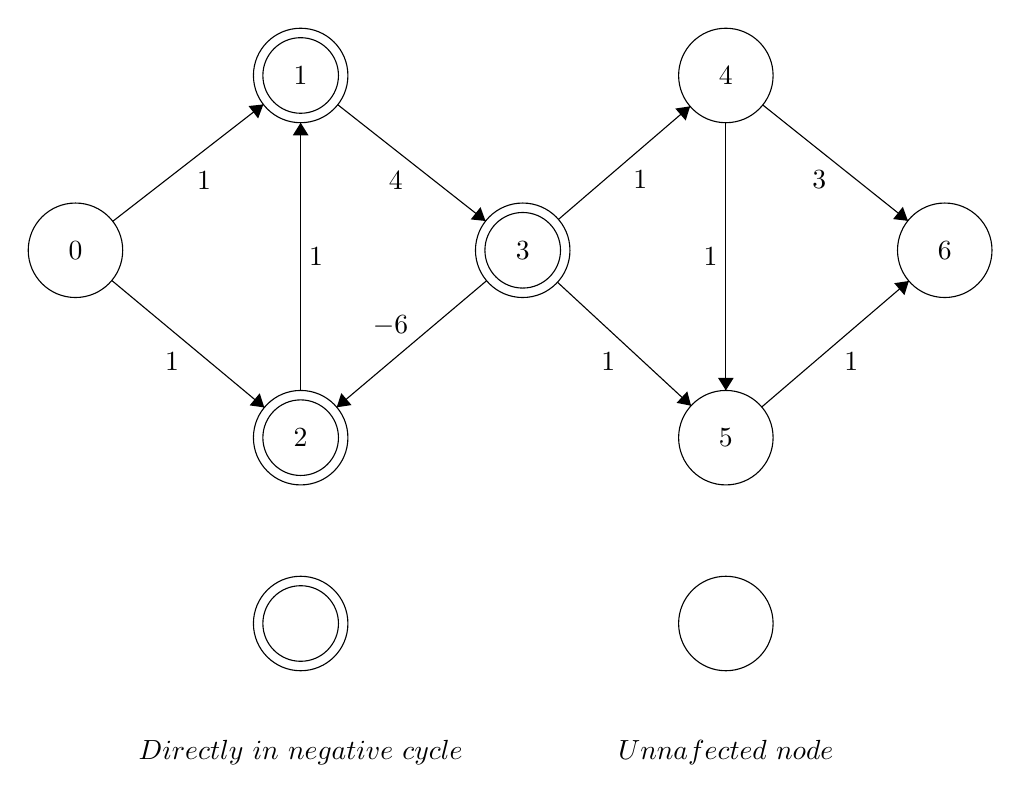
\begin{tikzpicture}[scale=0.2]
    \tikzstyle{every node}+=[inner sep=0pt]
    \draw [black] (6.3,-24.7) circle (3);
    \draw (6.3,-24.7) node {$0$};
    \draw [black] (20.6,-13.6) circle (3);
    \draw (20.6,-13.6) node {$1$};
    \draw [black] (20.6,-13.6) circle (2.4);
    \draw [black] (20.6,-36.6) circle (3);
    \draw (20.6,-36.6) node {$2$};
    \draw [black] (20.6,-36.6) circle (2.4);
    \draw [black] (34.7,-24.7) circle (3);
    \draw (34.7,-24.7) node {$3$};
    \draw [black] (34.7,-24.7) circle (2.4);
    \draw [black] (47.6,-13.6) circle (3);
    \draw (47.6,-13.6) node {$4$};
    \draw [black] (47.6,-36.6) circle (3);
    \draw (47.6,-36.6) node {$5$};
    \draw [black] (61.5,-24.7) circle (3);
    \draw (61.5,-24.7) node {$6$};
    \draw [black] (20.6,-48.4) circle (3);
    \draw [black] (20.6,-48.4) circle (2.4);
    \draw [black] (47.6,-48.4) circle (3);
    \draw (20.6,-56.6) node {$Directly\mbox{ }in\mbox{ }negative\mbox{ }cycle$};
    \draw (47.6,-56.6) node {$Unnafected\mbox{ }node$};
    \draw [black] (8.67,-22.86) -- (18.23,-15.44);
    \fill [black] (18.23,-15.44) -- (17.29,-15.54) -- (17.9,-16.33);
    \draw (14.46,-19.65) node [below] {$1$};
    \draw [black] (8.61,-26.62) -- (18.29,-34.68);
    \fill [black] (18.29,-34.68) -- (18,-33.78) -- (17.36,-34.55);
    \draw (12.44,-31.14) node [below] {$1$};
    \draw [black] (20.6,-33.6) -- (20.6,-16.6);
    \fill [black] (20.6,-16.6) -- (20.1,-17.4) -- (21.1,-17.4);
    \draw (21.1,-25.1) node [right] {$1$};
    \draw [black] (22.96,-15.46) -- (32.34,-22.84);
    \fill [black] (32.34,-22.84) -- (32.02,-21.96) -- (31.4,-22.74);
    \draw (26.64,-19.65) node [below] {$4$};
    \draw [black] (32.41,-26.63) -- (22.89,-34.67);
    \fill [black] (22.89,-34.67) -- (23.83,-34.53) -- (23.18,-33.77);
    \draw (26.31,-30.16) node [above] {$-6$};
    \draw [black] (47.6,-16.6) -- (47.6,-33.6);
    \fill [black] (47.6,-33.6) -- (48.1,-32.8) -- (47.1,-32.8);
    \draw (47.1,-25.1) node [left] {$1$};
    \draw [black] (36.97,-22.74) -- (45.33,-15.56);
    \fill [black] (45.33,-15.56) -- (44.39,-15.7) -- (45.05,-16.46);
    \draw (42.16,-19.64) node [below] {$1$};
    \draw [black] (36.91,-26.73) -- (45.39,-34.57);
    \fill [black] (45.39,-34.57) -- (45.15,-33.66) -- (44.47,-34.39);
    \draw (40.13,-31.14) node [below] {$1$};
    \draw [black] (49.94,-15.47) -- (59.16,-22.83);
    \fill [black] (59.16,-22.83) -- (58.84,-21.94) -- (58.22,-22.72);
    \draw (53.54,-19.64) node [below] {$3$};
    \draw [black] (49.88,-34.65) -- (59.22,-26.65);
    \fill [black] (59.22,-26.65) -- (58.29,-26.79) -- (58.94,-27.55);
    \draw (55.56,-31.14) node [below] {$1$};
    \end{tikzpicture}
\end{center}
\end{figure}

\textbf{Algorithms:} Bellman-Ford, Floyd-Warshall

\subsubsection{Strongly connected components}
Strongly connected components (SCCs) can be thought of as \textsf{self-contained cycles} within a directed graph where every vertex in a given cycle can reach every other vertex in the same cycle.

\begin{figure}[H]
\begin{center}
    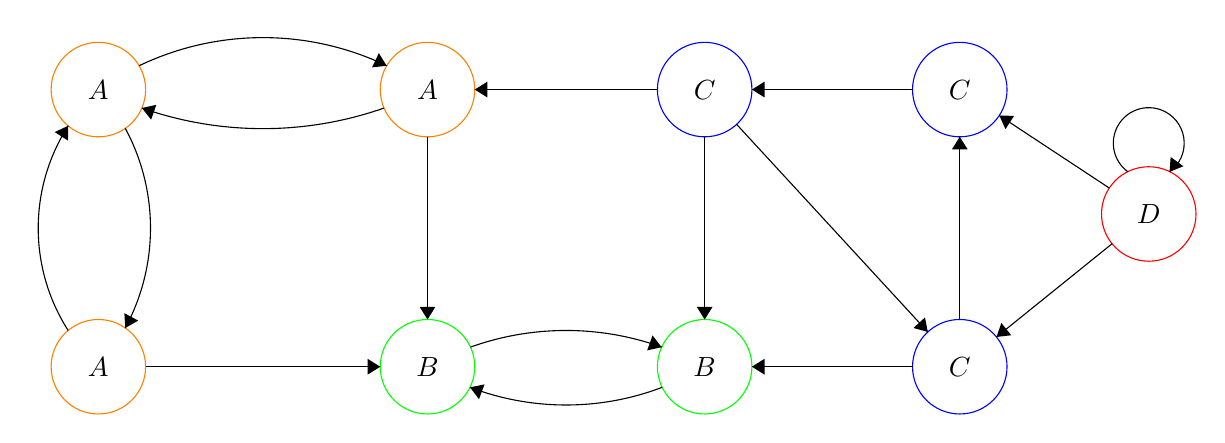
\begin{tikzpicture}[scale=0.2]
    \tikzstyle{every node}+=[inner sep=0pt]
    \draw [orange] (7.6,-22.4) circle (3);
    \draw (7.6,-22.4) node {$A$};
    \draw [orange] (7.6,-40) circle (3);
    \draw (7.6,-40) node {$A$};
    \draw [orange] (28.5,-22.4) circle (3);
    \draw (28.5,-22.4) node {$A$};
    \draw [green] (28.5,-40) circle (3);
    \draw (28.5,-40) node {$B$};
    \draw [blue] (46.1,-22.4) circle (3);
    \draw (46.1,-22.4) node {$C$};
    \draw [green] (46.1,-40) circle (3);
    \draw (46.1,-40) node {$B$};
    \draw [blue] (62.3,-22.4) circle (3);
    \draw (62.3,-22.4) node {$C$};
    \draw [blue] (62.3,-40) circle (3);
    \draw (62.3,-40) node {$C$};
    \draw [red] (74.3,-30.3) circle (3);
    \draw (74.3,-30.3) node {$D$};
    \draw [black] (10.6,-40) -- (25.5,-40);
    \fill [black] (25.5,-40) -- (24.7,-39.5) -- (24.7,-40.5);
    \draw [black] (5.685,-37.701) arc (-147.33564:-212.66436:12.045);
    \fill [black] (5.68,-24.7) -- (4.83,-25.1) -- (5.67,-25.64);
    \draw [black] (10.187,-20.887) arc (115.60514:64.39486:18.196);
    \fill [black] (25.91,-20.89) -- (25.41,-20.09) -- (24.98,-20.99);
    \draw [black] (28.5,-25.4) -- (28.5,-37);
    \fill [black] (28.5,-37) -- (29,-36.2) -- (28,-36.2);
    \draw [black] (9.308,-24.859) arc (28.34814:-28.34814:13.355);
    \fill [black] (9.31,-37.54) -- (10.13,-37.07) -- (9.25,-36.6);
    \draw [black] (25.741,-23.572) arc (-70.67485:-109.32515:23.24);
    \fill [black] (10.36,-23.57) -- (10.95,-24.31) -- (11.28,-23.37);
    \draw [black] (43.1,-22.4) -- (31.5,-22.4);
    \fill [black] (31.5,-22.4) -- (32.3,-22.9) -- (32.3,-21.9);
    \draw [black] (46.1,-25.4) -- (46.1,-37);
    \fill [black] (46.1,-37) -- (46.6,-36.2) -- (45.6,-36.2);
    \draw [black] (43.404,-41.307) arc (-69.15663:-110.84337:17.154);
    \fill [black] (31.2,-41.31) -- (31.77,-42.06) -- (32.12,-41.12);
    \draw [black] (59.3,-22.4) -- (49.1,-22.4);
    \fill [black] (49.1,-22.4) -- (49.9,-22.9) -- (49.9,-21.9);
    \draw [black] (59.3,-40) -- (49.1,-40);
    \fill [black] (49.1,-40) -- (49.9,-40.5) -- (49.9,-39.5);
    \draw [black] (62.3,-37) -- (62.3,-25.4);
    \fill [black] (62.3,-25.4) -- (61.8,-26.2) -- (62.8,-26.2);
    \draw [black] (71.79,-28.65) -- (64.81,-24.05);
    \fill [black] (64.81,-24.05) -- (65.2,-24.91) -- (65.75,-24.07);
    \draw [black] (71.97,-32.19) -- (64.63,-38.11);
    \fill [black] (64.63,-38.11) -- (65.57,-38) -- (64.94,-37.22);
    \draw [black] (72.977,-27.62) arc (234:-54:2.25);
    \fill [black] (75.62,-27.62) -- (76.5,-27.27) -- (75.69,-26.68);
    \draw [black] (31.226,-38.755) arc (109.75883:70.24117:17.968);
    \fill [black] (43.37,-38.76) -- (42.79,-38.01) -- (42.45,-38.96);
    \draw [black] (48.13,-24.61) -- (60.27,-37.79);
    \fill [black] (60.27,-37.79) -- (60.09,-36.87) -- (59.36,-37.54);
    \end{tikzpicture}
\end{center}
\end{figure}

\textbf{Algorithms:} Tarjan's and Kosaraju's algorithm

\subsubsection{Traveling salesman problem}

''Given a list of cities and the distances between each pair of cities, what is the shortest possible route that visists each city exactly once and returns to the origin city?''

\begin{figure}[H]
\begin{center}
    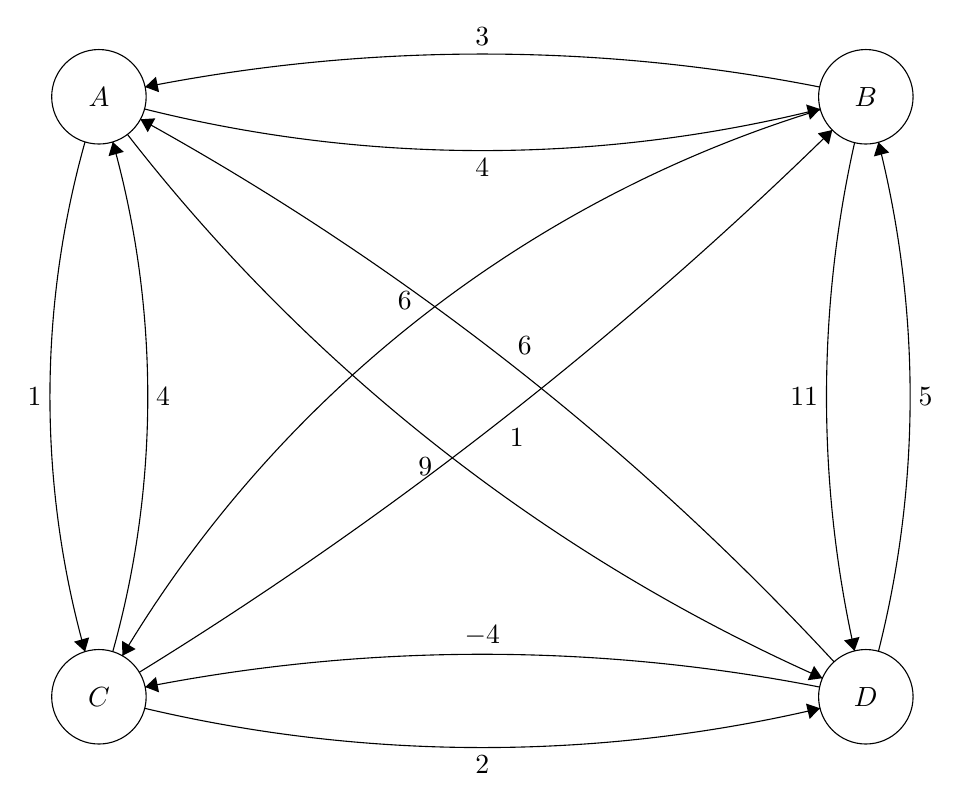
\begin{tikzpicture}[scale=0.2]
    \tikzstyle{every node}+=[inner sep=0pt]
    \draw [black] (13.2,-11.3) circle (3);
    \draw (13.2,-11.3) node {$A$};
    \draw [black] (61.9,-11.3) circle (3);
    \draw (61.9,-11.3) node {$B$};
    \draw [black] (13.2,-49.4) circle (3);
    \draw (13.2,-49.4) node {$C$};
    \draw [black] (61.9,-49.4) circle (3);
    \draw (61.9,-49.4) node {$D$};
    \draw [black] (59.003,-12.077) arc (-75.95717:-104.04283:88.411);
    \fill [black] (59,-12.08) -- (58.11,-11.79) -- (58.35,-12.76);
    \draw (37.55,-15.22) node [below] {$4$};
    \draw [black] (16.136,-48.782) arc (101.11037:78.88963:111.128);
    \fill [black] (16.14,-48.78) -- (17.02,-49.12) -- (16.82,-48.14);
    \draw (37.55,-46.2) node [above] {$-4$};
    \draw [black] (14.081,-14.167) arc (15.64211:-15.64211:60.018);
    \fill [black] (14.08,-14.17) -- (13.81,-15.07) -- (14.78,-14.8);
    \draw (16.8,-30.35) node [right] {$4$};
    \draw [black] (61.185,-46.487) arc (-167.37456:-192.62544:73.826);
    \fill [black] (61.18,-46.49) -- (61.5,-45.6) -- (60.52,-45.82);
    \draw (58.9,-30.35) node [left] {$11$};
    \draw [black] (16.135,-10.679) arc (101.17144:78.82856:110.532);
    \fill [black] (16.13,-10.68) -- (17.02,-11.01) -- (16.82,-10.03);
    \draw (37.55,-8.08) node [above] {$3$};
    \draw [black] (62.702,-14.191) arc (14.19594:-14.19594:65.892);
    \fill [black] (62.7,-14.19) -- (62.41,-15.09) -- (63.38,-14.84);
    \draw (65.21,-30.35) node [right] {$5$};
    \draw [black] (58.992,-50.135) arc (-76.74004:-103.25996:93.48);
    \fill [black] (58.99,-50.13) -- (58.1,-49.83) -- (58.33,-50.81);
    \draw (37.55,-53.13) node [below] {$2$};
    \draw [black] (12.317,-46.533) arc (-164.32039:-195.67961:59.88);
    \fill [black] (12.32,-46.53) -- (12.58,-45.63) -- (11.62,-45.9);
    \draw (9.59,-30.35) node [left] {$1$};
    \draw [black] (59.142,-48.219) arc (-113.92458:-142.15047:114.901);
    \fill [black] (59.14,-48.22) -- (58.61,-47.44) -- (58.21,-48.35);
    \draw (33.93,-34.18) node [below] {$9$};
    \draw [black] (15.839,-12.726) arc (61.12932:42.79563:175.501);
    \fill [black] (15.84,-12.73) -- (16.3,-13.55) -- (16.78,-12.67);
    \draw (40.25,-27.69) node [above] {$6$};
    \draw [black] (14.689,-46.796) arc (149.13758:106.93747:78.164);
    \fill [black] (14.69,-46.8) -- (15.53,-46.37) -- (14.67,-45.85);
    \draw (32.62,-24.83) node [above] {$6$};
    \draw [black] (59.77,-13.413) arc (-45.56883:-58.35612:250.875);
    \fill [black] (59.77,-13.41) -- (58.85,-13.62) -- (59.55,-14.33);
    \draw (39.73,-32.35) node [below] {$1$};
    \end{tikzpicture}
\end{center}    
\end{figure}

One possible solution is the next: 

\begin{figure}[H]
\begin{center}
    \begin{tikzpicture}[scale=0.2]
    \tikzstyle{every node}+=[inner sep=0pt]
    \draw [black] (13.2,-11.3) circle (3);
    \draw (13.2,-11.3) node {$A$};
    \draw [black] (61.9,-11.3) circle (3);
    \draw (61.9,-11.3) node {$B$};
    \draw [black] (13.2,-49.4) circle (3);
    \draw (13.2,-49.4) node {$C$};
    \draw [black] (61.9,-49.4) circle (3);
    \draw (61.9,-49.4) node {$D$};
    \draw [black] (16.136,-48.782) arc (101.11037:78.88963:111.128);
    \fill [black] (16.14,-48.78) -- (17.02,-49.12) -- (16.82,-48.14);
    \draw (37.55,-46.2) node [above] {$-4$};
    \draw [black] (16.135,-10.679) arc (101.17144:78.82856:110.532);
    \fill [black] (16.13,-10.68) -- (17.02,-11.01) -- (16.82,-10.03);
    \draw (37.55,-8.08) node [above] {$3$};
    \draw [black] (59.142,-48.219) arc (-113.92458:-142.15047:114.901);
    \fill [black] (59.14,-48.22) -- (58.61,-47.44) -- (58.21,-48.35);
    \draw (33.93,-34.18) node [below] {$9$};
    \draw [black] (59.77,-13.413) arc (-45.56883:-58.35612:250.875);
    \fill [black] (59.77,-13.41) -- (58.85,-13.62) -- (59.55,-14.33);
    \draw (39.73,-32.35) node [below] {$1$};
    \end{tikzpicture}
\end{center}        
\end{figure}

\textbf{Algorithms: } Held-Karp, branch and bound and many approximation algorithms.